\documentclass[11pt]{article}
\usepackage[utf8]{inputenc}
\usepackage{amsmath}
\usepackage{amssymb}
\usepackage{graphicx}
\usepackage{indentfirst}
\usepackage{hyperref}
\let\oldemptyset\emptyset
\let\emptyset\varnothing


\title{\textbf{Handout: The basics of Probability Theory and Set Theory}}

\author{Leonardo S. Barone}
\date{}

\begin{document}

\maketitle

\section{Set Theory}

Basic notions and notation of set theory.

\subsection{First concepts and notation}

	\begin{itemize}
		\item Sets are a list or collection of objects.
		\item These objects are elements.
		\item $\emptyset$ is the empty set.
		\item $p \in A$: is p is an element in the set $A$.
		\item $A \subset B$: $A$ is a subset of $B$ 
	\end{itemize}


\subsection{Set Theory - operations}

	\begin{itemize}
		\item $A \cup B$: union of $A$ and $B$.
		\begin{itemize}
			\item $p \in (A \cup B$): p is an element of $A$ \textbf{OR} $B$.
		\end{itemize}
		\item $A \cap B$: intersection of $A$ an $B$.
		\begin{itemize}
			\item $p \in (A \cup B$): p is an element of $A$ \textbf{AND} $B$.
		\end{itemize}
		\item If $A \cap B$ is equal to $\emptyset$, then A and B are \textbf{disjoint} sets.
		\item $A^c$ ($A'$, \textasciitilde$A$ or simply \emph{not A}) is the set of all elements that does not belong to $A$. $A_c$ is the complement of $A$. 

	\end{itemize}

\subsection{Venn Diagrams}
 We can represent sets with diagrams. These are called ``Venn Diagrams''. Check Figure 1 and locate the following sets as a quick exercise:\\


\begin{tabular}{llll}
	1) $A \cup B$ & 5) $(A \cup B) \cup C$ & 9) $A^c$ & 13) $((A \cap B) \cap C)^c$\\
	2) $A \cap B$ & 6) $(A \cap B) \cap C$ & 10) $(A \cap B)^c$ & 14) $((A \cup B) \cap C)^c$\\
	3) $A \cup C$ & 7) $(A \cup B) \cap C$ & 11) $(A \cup C)^c$ &\\
	4) $A \cap C$ & 8) $(A \cap B) \cup C$ & 12) $((A \cup B) \cup C)^c$ &\\
\end{tabular}

\begin{figure}[htp]
\centering
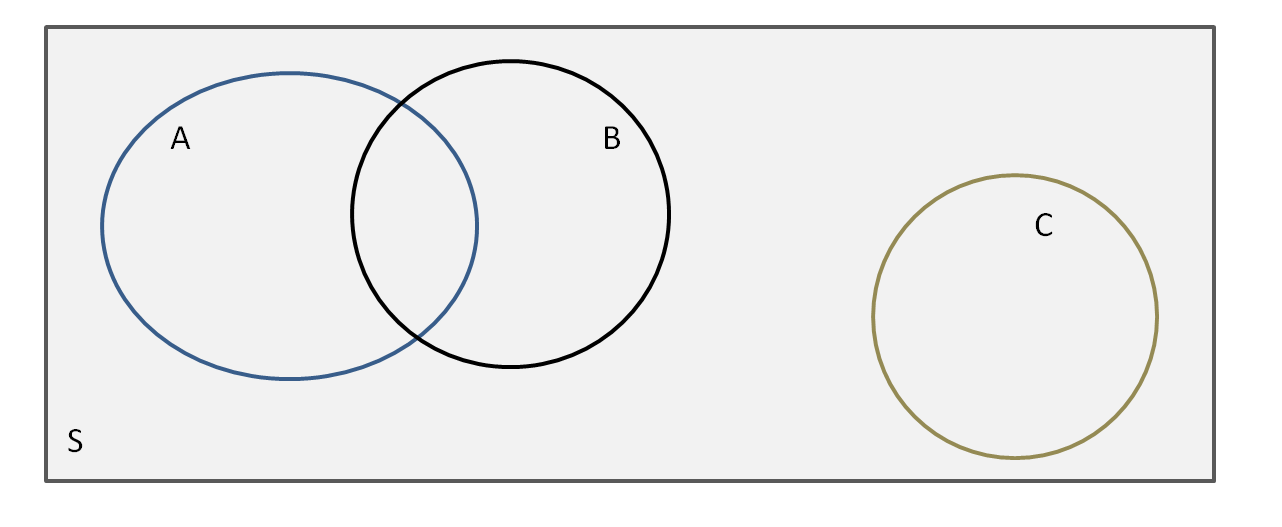
\includegraphics[scale=0.50]{venn.png}
\caption{Venn Diagrams}
\label{}
\end{figure}


\pagebreak

\section{Introduction to Probability - Part I}

	Basic Notions of probability,
	
	\subsection{Probabilty}
	Probability is a formal model of uncertainty.

	\begin{enumerate}
	\item Objetive probability:
		\begin{itemize}
			\item Classical - theory driven. Ex: dice or coin.
			\item Empirical - observation driven. Ex: voting for winner in presidential election.
		\end{itemize}
	\item Subjective probability - belief driven. Ex: educated guess about the happening of an event.
	\end{enumerate}

	\subsection{Coins, dices, cards and legislators.}
	
	Let's see how probability works for coins, dices, cards and legislators in this handout.
	
		\begin{itemize}
			\item Toss a coin. What is the probability of getting a head?
			\item Toss a coin. What is the probability of getting a head?
		\end{itemize}
	\[P(Head) = P(Tail) = 1/2	\]
	How do we know it without actually tossing a coin?

	\subsection{First Definitions}
	\begin{itemize}
		\item \emph{Sample space (S)}: the set of all possible outcomes.
		\item \emph{Outcome}: is an element of the sample space.
		\item \emph{Event}: any collection of possible outcomes.
		\item The empty set $\emptyset$ and the sample space S are also events.	
		\item \emph{Probability of event A}:
			\[P(A) = \frac{\text{Number of outcomes in event A}}
			{\text{Number of outcomes in the sample space}}\]		
	\end {itemize}


	\subsection{Axioms and theorems of probability (1)}
	\begin{itemize}
		\item For every event A, $0 \leq P(A) \leq 1$
		\item $P(S) = 1$
		\item $P(\emptyset) = 0$
	\end{itemize}


	\subsection{Coin}
	Toss a coin. What is the probability of getting a head?\\
	
	Sample Space = \emph{\{Head,Tail\}} -- 2 possible outcomes\\
	
	Event A = \emph{\{Head\}} -- 1 possible outcome\\
	
	\[P(A) = \frac{\text{Number of outcomes in event A}}
	{\text{Number of outcomes in the sample space}} = \frac{1}{2}\]


	\subsection{Dice - quick exercise}
	Roll a 6-side dice.\\
	
	What is the probability of getting a 5?\\
	\[P(5) = ?	\]\\
	
	What is the probability of getting an even number?\\
	\[P(even) = ?	\]\\
	
	What is the probability of getting a prime number?\\
	\[P(prime) = ?	\]\\	


	\subsection{Dice - quick exercise - answers}

	Roll a 6-side dice.\\
	
	What is the probability of getting a 5?\\
	\[P(5) = 1/6	\]\\
	
	What is the probability of getting an even number?\\
	\[P(even) = \frac{\#\{2, 4, 6\}}{6} = \frac{3}{6} = \frac{1}{2}	\]\\
		
	What is the probability of getting a prime number?\\
	\[P(prime) = \frac{\#\{2, 3, 5\}}{6} = \frac{3}{6} = \frac{1}{2}	\]\\	

	\subsection{Random legislator - quick exercise}

	Choose a Legislative House of your choice, in any country/state/province/city in the world. Choose a political party and call it Party A. (A nice and not-up-to-date visualization of Brazilian Câmara dos Deputados can be found \href{http://g1.globo.com/politica/eleicoes/2014/nova-composicao-da-camara.html}{here}. Let's get a random legislator from that House.\\
	
	What is the probability of getting a legislator from the Party A?
	\[P(\text{party A}) = ?\]
	
	What is the probability of getting a woman?
	\[P(woman) = ?\]

	\subsection{Question - classical or empirical?}

	What is the difference between the dice and the random legislator examples? Did we have to actually roll the dices to get calculate the probabilities of getting a 5, an even or prime number? Can I guess the probability of choosing at random a woman or a legislator from Party A without observing and counting legislators?\\

	Let's get frustrated a little bit. Let's toss a coin 10 times (or toss 10 coins) and check how many heads we get. There "should" be 5 heads, rigth?\\


	Now let's do it 100 times. And 1000. And 1000000.
	
	\begin{verbatim}

	 *install new ado (aka package w/ new functions) using the command findit
	 findit heads

	 * toss 10 a fair coin
	 heads, flips(10)

	 * toss 100 a fair coin
	 heads, flips(100)
	 
	 * toss 1000 a fair coin
	 heads, flips(1000)
	 
	 * toss 1000000 a fair coin
	 heads, flips(1000000)

	\end{verbatim}
	
	What if we use a biased coin?

	\begin{verbatim}

	 * toss 100 a biased coin w/ P(Head) = 0.3
	heads, flips(100) prob(.3)	 
	
	 * toss 1000 a biased coin w/ P(Head) = 0.3
	heads, flips(1000) prob(.3)	 

	\end{verbatim}

\pagebreak
\section{Introduction to Probability - Part II}

	\subsection{Single or Compound events? Independence and Exclusivity}

	An event can be simple (a single outcome) or compound (two or more single events).\\

	The relation between the events that form a compound event can be defined as:
	
	\begin{itemize}
		\item \emph{Independent}: two events are independent if the probability that one occurs does not change as a consequence of the other event’s occurring.
		\item \emph{Mutual exclusivity}: two events are mutually exclusive when one cannot occur if the  other has occurred.
		\item \emph{Collective exhaustivity}: the set of collective exhaustive events is the whole sample space.
	\end {itemize}


	\subsection{Axioms and theorems of probability (2)}
	\begin{itemize}
		\item  If $A$ and $B$ are mutually exclusive, then:
	\[P(A \cup B) = P(A) + P (B)\]
		\item  If $A_1$, $A_2$, ... is a sequence of mutually exclusive events, then:
	\[P(A_1 \cup A_2 \cup ... \cup A_n) = P(A_1) + P (A_2) + ... + P(A_n)\]
	\end{itemize}


	\subsection{Dices and mutually exclusive events}

	Roll a 6-side dice.\\
	
	What's is the probability of getting a 5 \textbf{OR} a 6?\\
	\[P(\text{5 or 6}) = P(5 \cup 6) = ?\]\\
	
	What's is the probability of getting a prime \textbf{OR} an odd number?\\
	\[P(\text{prime or odd}) = P(\text{prime }\cup\text{ odd}) = ?\]

	\subsection{Dices and mutually exclusive events - answers}

	Roll a 6-side dice.\\
	
	What's is the probability of getting a 5 \textbf{OR} a 6?\\
	\[P(\text{5 or 6}) = P(5 \cup 6) = \frac{\#\{5, 6\}}{6} = \frac{2}{6} = \frac{1}{3} = \frac{1}{6} + \frac{1}{6} = P(5) + P(6)\]\\ 
	since 5 and 6 are mutually exclusive events.\\
	
	What's is the probability of getting a prime \textbf{OR} an odd number?\\

	\textbf{Beware!!!} This is not true for events that are not mutually exclusive (note that 3 and 5 are both prime and odd).

	\[P(\text{prime}) + P(\text{odd}) = \frac{\#\{2, 3, 5\}}{6} + \frac{\#\{1, 3, 5\}}{6} = \frac{3}{6} + \frac{3}{6} = \frac{6}{6} = 1\]
	
	\[P(\text{prime or odd}) = P(\text{prime }\cup\text{ odd}) = \frac{\#\{1, 2, 3, 5\}}{6} = \frac{4}{6} \neq P(\text{prime}) + P(\text{odd})\]


	\subsection{Mutually exclusive events - random legislator}

	Let's go back to the Legislative House example.\\
	
	What's is the probability of getting a legislator from Party A \textbf{OR} B?
	\[P(\text{A or B}) = P(A \cup B) = ?\]
	
	What's is the probability of getting a legislator from Party A \textbf{OR} a woman (W)?
	\[P(\text{A or W}) = P(A \cup W) =?\]


	\subsection{Mutually exclusive events - random legislator - answers}
	
	Let's go back to the Legislative House example.\\
	
	What's is the probability of getting a legislator from Party A \textbf{OR} B?
	\[P(\text{A or B}) = P(A \cup B) = P(A) + P(B)\]
	
	What's is the probability of getting a legislator from Party A \textbf{OR} a woman (W)?\\
	
	If there is at leat a woman on party A, the events are not mutually excluise and \[P(\text{A or W}) = P(A \cup W) \neq P(A) + P(W)\]
	
	If it is a all-men party, being a woman and beloging to party A are mutually exclusive and
	\[P(A \cup W) = P(A) + P(W)\]


	\subsection{Axioms and theorems of probability (3)}
	$A^c$ is the complementary event of A.
	\begin{itemize}
		\item  $P(A^c) = 1 - P(A)$
		\item  $P(A \cup A^c) = P(A) + P(A^c) = 1$ (because they are mutually exclusive)
	\end{itemize}


	\subsection{Complementary event (not A, ~A, A' or $A^c$)}
	What is the probability of \textbf{NOT} getting a 5 on a 6-side dice?
	\[P(\text{not 5}) = P\text{(\{1,2,3,4,6\})} = \frac{\#\{1, 2, 3, 4, 6\}}{6} =  5/6	\]

	Or, more elegantly:
	\[P(\text{not 5}) = 1 - P(5) = 1 - \frac{1}{6} = \frac{5}{6}\]

\pagebreak
\section{Introduction to Probability - Part III}

	\subsection{Axioms and theorems of probability (4)}
	\begin{itemize}
		\item $P(A \cap B)$ is the the probability of $A$ \textbf{AND} $B$ happening at the same time.																																																																																																																		
		\item  $P(A \cup B) = P(A) + P(B) - P(A \cap B)$ 
	\end{itemize}


\end{document}
